\documentclass[english,xcolor=dvipsnames]{beamer}
\usepackage[autolinebreaks,useliterate]{mcode}
\usepackage[orientation=landscape,size=custom,width=16,height=9,scale=0.48,debug]{beamerposter}
\usepackage[T1]{fontenc}
\usepackage[latin9]{inputenc}
\usepackage{amsthm}
\usepackage{amsmath}
\usepackage{amssymb}
\usepackage{bookmark}
\usepackage{graphics,graphicx}
\usepackage{pstricks,pst-node,pst-tree}
\usefonttheme{serif}
\usepackage{palatino}
\usepackage{tikz}
\usetikzlibrary{shapes,arrows}
\usetikzlibrary{positioning}
%\usepackage[margin=.5cm]{geometry}

\definecolor{dgreen}{rgb}{0.,0.6,0.}
\definecolor{forest}{RGB}{34.,139.,34.}
\definecolor{byublue}{RGB}{0.,30.,76.}
\definecolor{dukeblue}{RGB}{0.,0.,156.}
%\usetheme{Ilmenau}
\usetheme{Warsaw}
\usecolortheme[named=dukeblue]{structure}
%\usecolortheme[named=RawSienna]{structure}
%\usecolortheme[named=byublue]{structure}
\setbeamertemplate{navigation symbols}{}
\setbeamertemplate{footline}{}
\setbeamercovered{transparent}

\newcommand{\be}{\begin{enumerate}}
\newcommand{\ee}{\end{enumerate}}
\newcommand{\bq}{\begin{quote}}
\newcommand{\eq}{\end{quote}}
\newcommand{\bd}{\begin{description}}
\newcommand{\ed}{\end{description}}
\newcommand{\bi}{\begin{itemize}}
\newcommand{\ei}{\end{itemize}}

\title[]{Unobserved Heterogeneity}
\author{Tyler Ransom}
\institute{Duke University}
\date{\today}

\begin{document}

\begin{frame}
   \titlepage
\end{frame}

\begin{frame}
\frametitle{Plan}
Introduce and discuss what unobserved heterogeneity is and why it's important
Go through different ways of correcting for unobs het 
      \bi 
      \item Some will be familiar
      \item You will see all of these (and more!) in your 2nd year
      \ei
\end{frame}

\begin{frame}
\frametitle{Unobserved Heterogeneity}

Researchers estimate models of the form $y_{i} = X_{i}\beta + \varepsilon_{i}$ where $y_{i}$ is some outcome variable and $\varepsilon_{i}$ is assumed to be uncorrelated with $X_{i}$.\\
In actuality, the $X_{i}$ and $\varepsilon_{i}$ are likely to be correlated
      \bi 
      \item This is usually because there are important variables explaining $y$ that are not included in $X$ (generally because of data limitations)
      \ei
\end{frame}

\begin{frame}
\frametitle{Unobserved Heterogeneity}
   \bi 
   \item What we mean by ``unobserved heterogeneity'' is that there is something the researcher can't observe, which is important in answering the research question
      \bi 
      \item The terms ``unobserved heterogeneity'' and ``endogeneity'' can be used interchangeably
      \item ``unobserved heterogeneity'' is the preferred term in 2nd year modules
      \ei
   \item Failing to correct for unobserved heterogeneity in some way will bias the estimates of the b (the parameters of interest)
   \item Correcting for unobserved heterogeneity is >50\% of the work in estimation
   \item We care about correcting for it because at the end of the day we want to recover a causal relationship for what we observe. We can't do this without making such a correction
   \item There are many, many ways to correct for unobserved heterogeneity (we'll discuss just a few today)
   \ei
\end{frame}

\begin{frame}
\frametitle{Examples of Unobserved Heterogeneity}
   IO
      \bi 
      \item Demand estimation: products have unobservable attributes that are correlated to their demand (e.g. iPad is cooler than other tablets, even above and beyond any observable trait like screen resolution or app market size)
      \ei
   Education
      \bi 
      \item Teacher quality: Teachers have interactions with students that can't be quantified in any test score metric, but these interactions directly affect student outcomes (and are correlated with $X$)
      \ei
   Labor
      \bi 
      \item Workers have unobservable attributes (like innate ability) that are directly related to productivity, but which are also correlated with $X$ (e.g. more ability $\Rightarrow$ more education)
      \ei
\end{frame}

\begin{frame}
\frametitle{Correcting for Unobserved Heterogeneity}
Ways of correcting for unobserved heterogeneity
      \bi 
      \item Instrumental Variables
      \item Fixed/Random Effects
      \item Nonlinear Models
         \bi 
         \item Nonparametric methods
         \item Parametric methods
         \ei
      \ei
We'll go through each of these (along with their relative advantages/disadvantages) in more depth
\end{frame}

\begin{frame}
\frametitle{Instrumental Variables}
   \bi 
   \item $y_{i} = X_{i}\beta + \varepsilon_{i}$
   \item $X_{i}$ correlated with $\varepsilon_{i}$
   \item Find some other set of variables $Z_{i}$ which is correlated with $X_{i}$ but not with $\varepsilon_{i}$
   \item Use GMM to estimate $\beta$
   \item Pros:
      \bi 
      \item Simple to implement
      \item Doesn't require panel data
      \item Doesn't necessarily require a linear model (though computation intensifies if instruments are used in a nonlinear case)
      \ei
   \item Cons:
      \bi 
      \item Hard to find instruments that satisfy the required conditions
      \item Overly simplistic in terms of describing behavior
      \ei
   \ei
\end{frame}

\begin{frame}
\frametitle{How estimates can change with panel data}
\begin{columns}[c]
\column{3in}
\centering{}
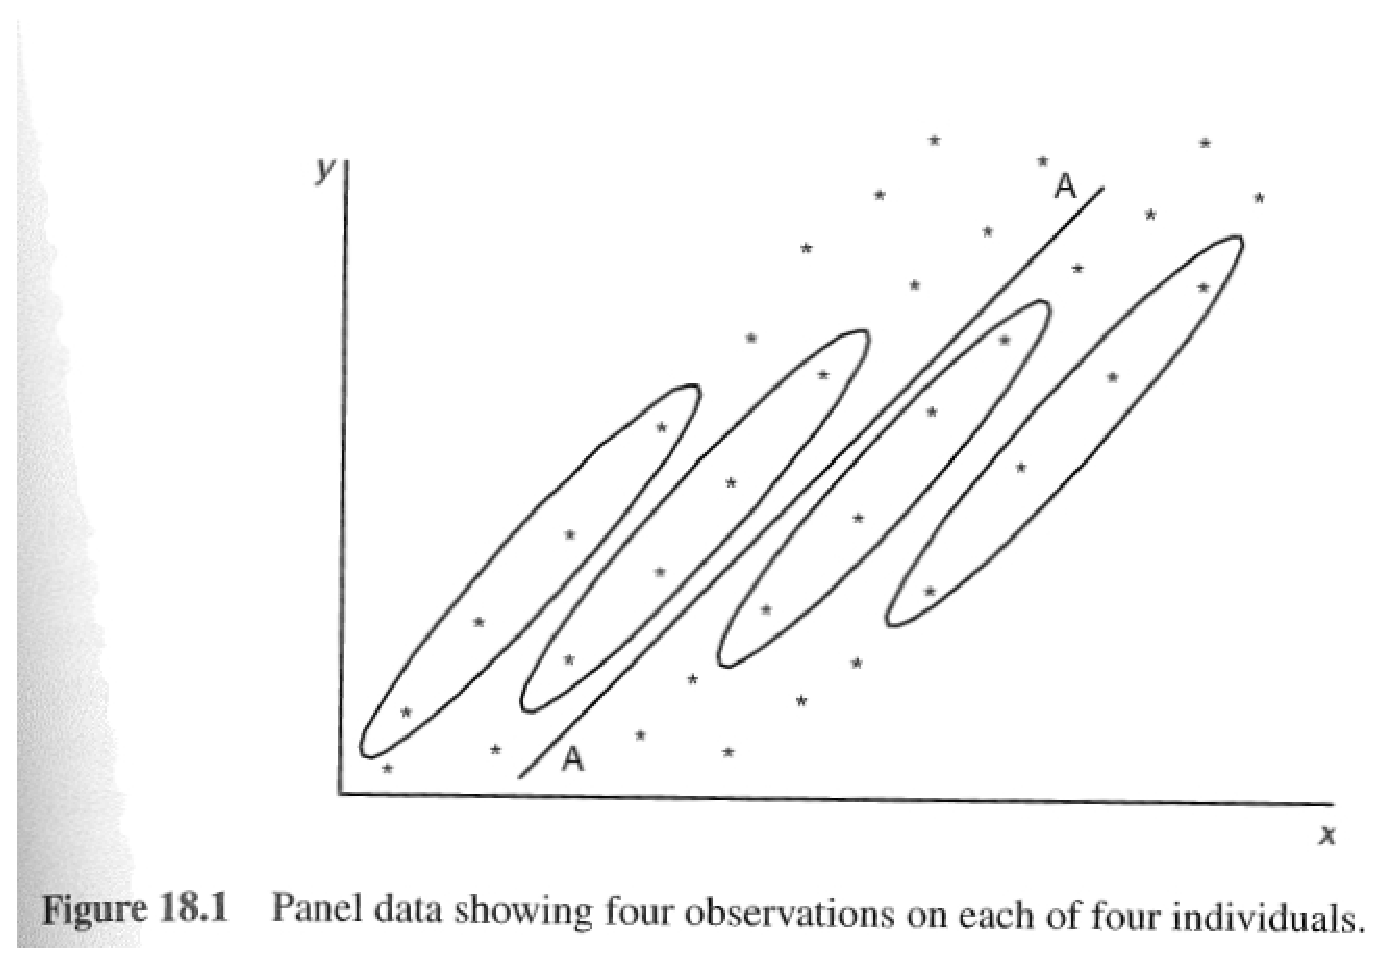
\includegraphics[scale=0.30]{FEKennedy1.eps} \\
\scriptsize{Source: Kennedy (2008)}
\column{3in}
\centering{}
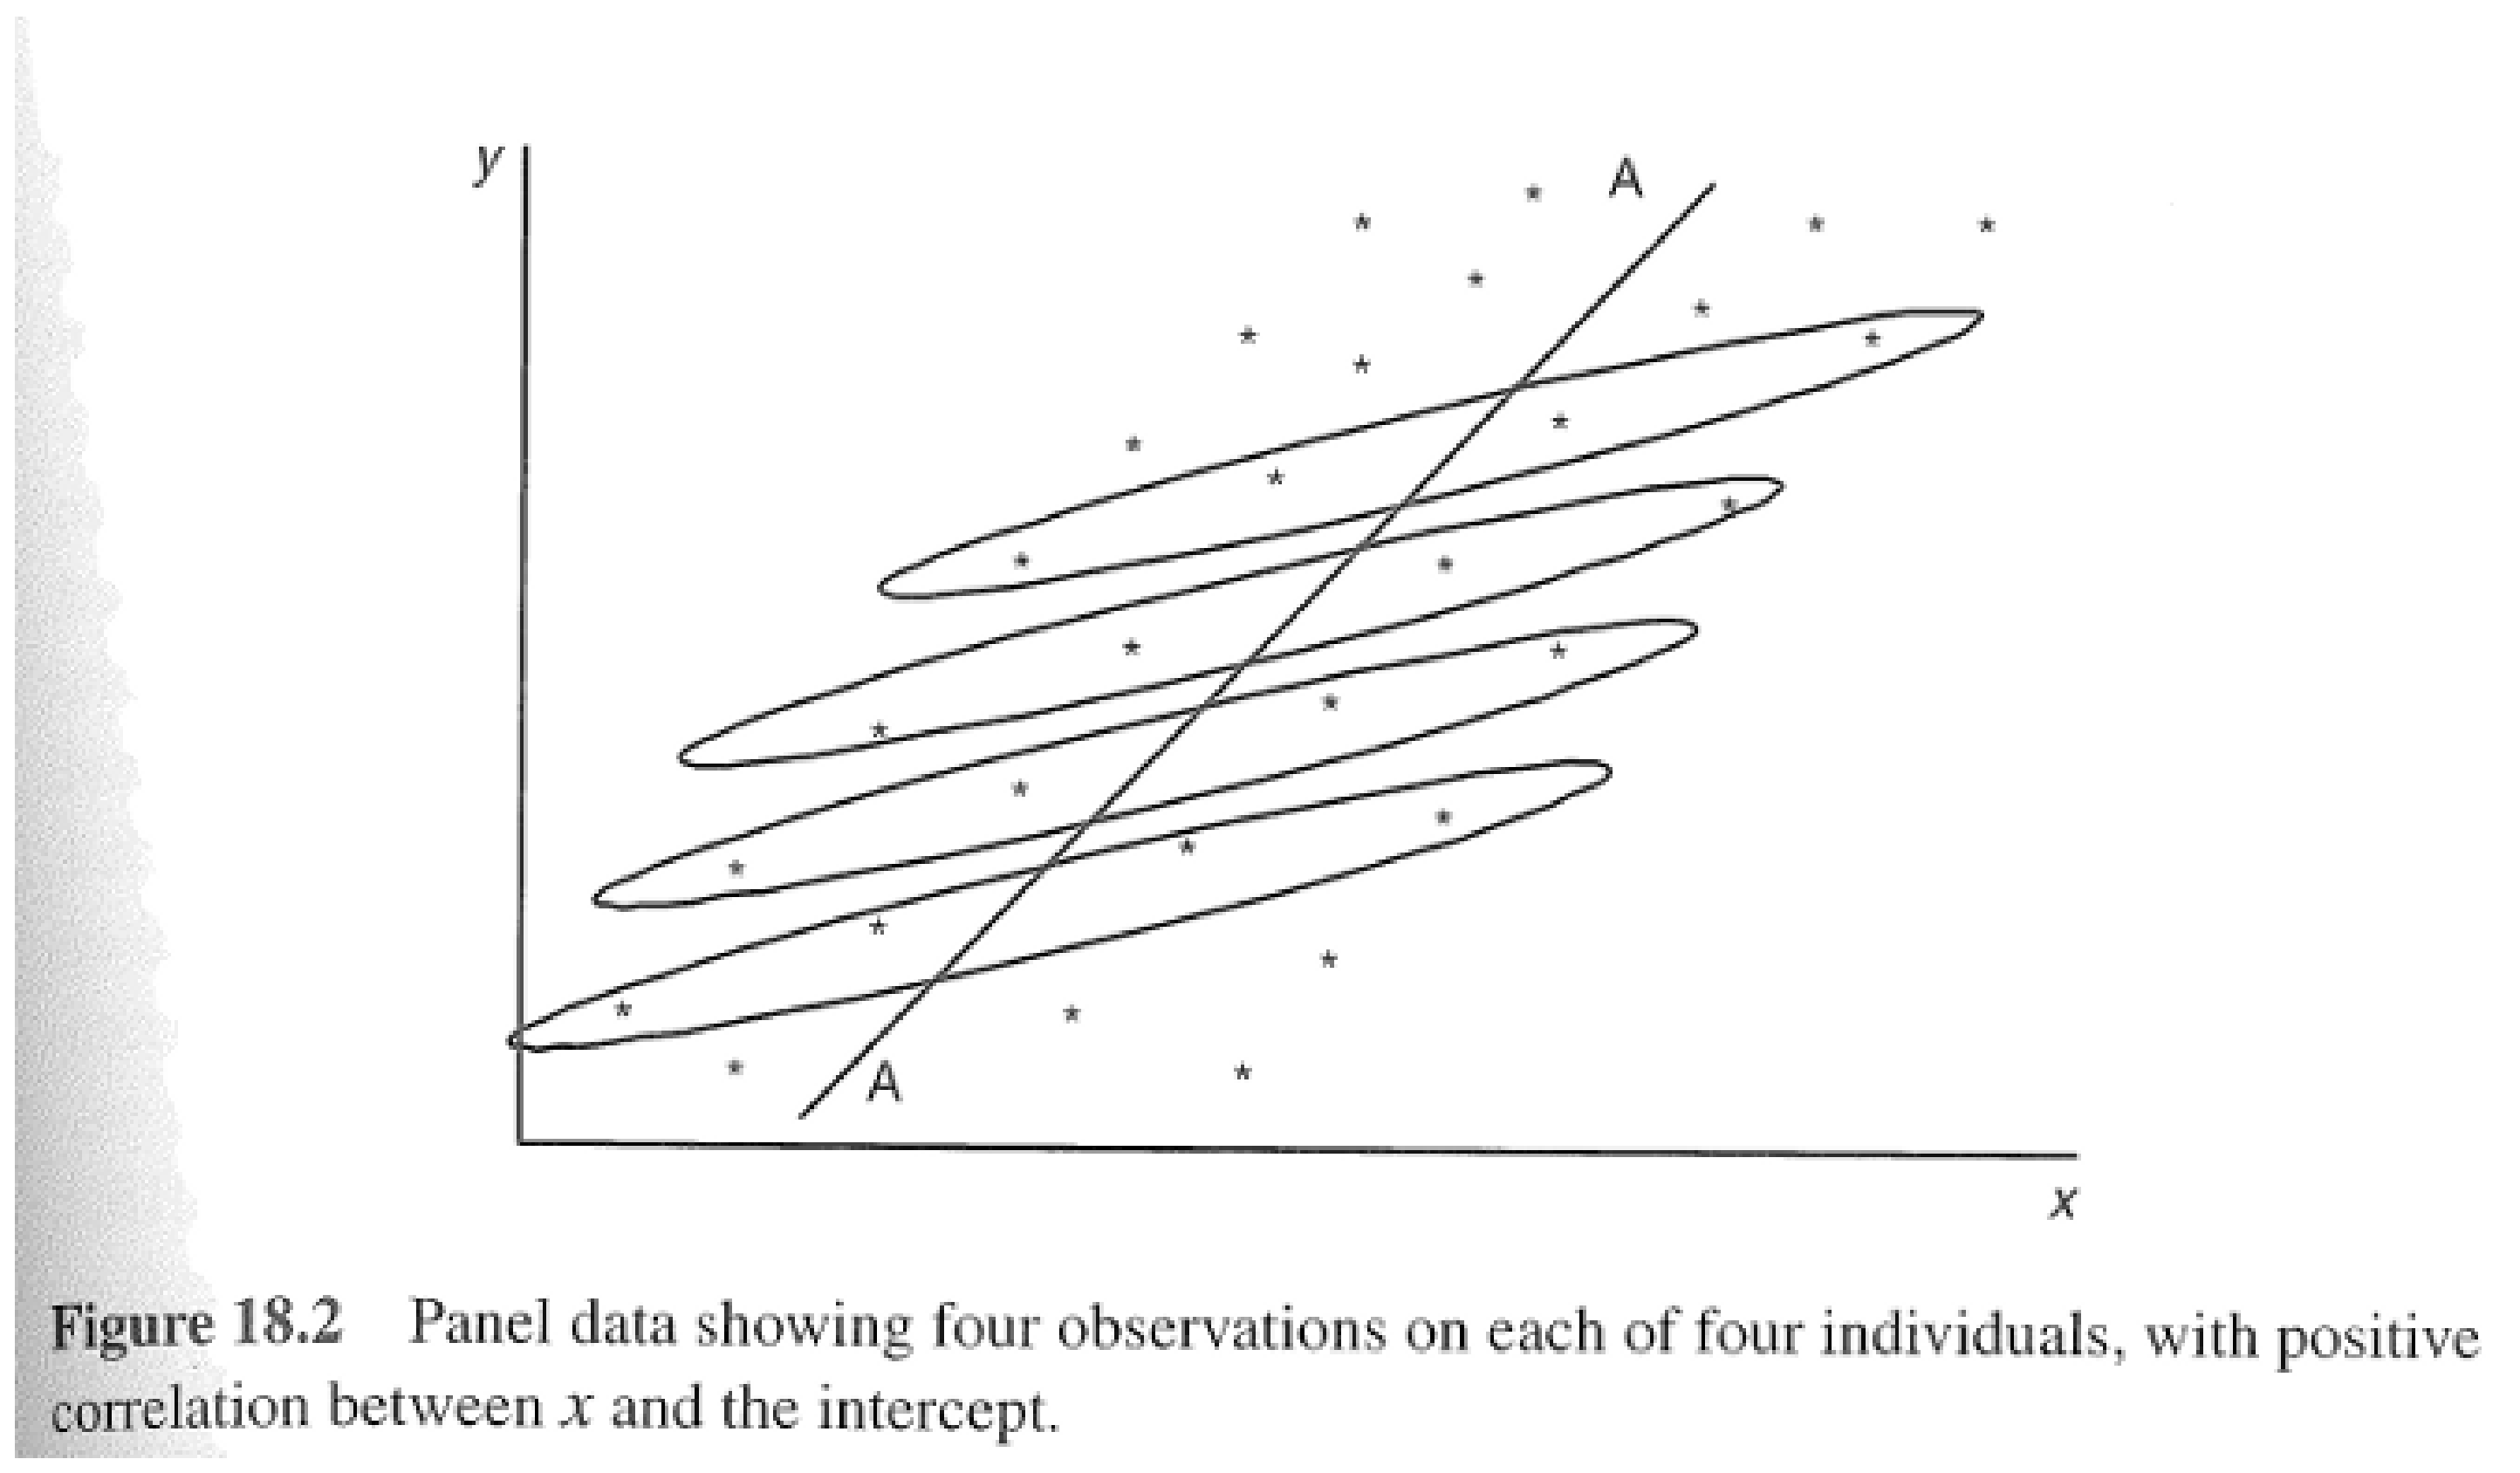
\includegraphics[scale=0.15]{FEKennedy2.eps} \\
\scriptsize{Source: Kennedy (2008)}
\end{columns}
%\vfill
\end{frame}

\begin{frame}
\frametitle{Fixed Effects, mathematically}
   \bi 
   \item $y_{it} = X_{it}\beta + \alpha_{i}+ \varepsilon_{it}$
   \item Decompose the error term into a persistent component ($\alpha_{i}$) and a transitory component ($\varepsilon_{it}$) -- both mean-zero
   \item Assume $\varepsilon_{it}$ is independent of $X_{it}$
   \item $\alpha_{i}$ can be correlated with $X_{it}$
   \item Use a difference within persons to recover beta: \[
         \hat{\beta} = \left(\sum_{i=1}^{N}\sum_{t=1}^{T}\ddot{X}_{it}^{\prime}\ddot{X}_{it}\right)^{-1} \sum_{i=1}^{N}\sum_{t=1}^{T}\ddot{X}_{it}^{\prime} \ddot{y}_{it}\] where $\ddot{X}_{it}=X_{it}-\overline{X}_{i}$ and $\ddot{y}_{it}=y_{it}-\overline{y}_{i}$
   \item The $\alpha_{i}$ disappears because it is time-invariant
   \ei
\end{frame}

\begin{frame}
\frametitle{Fixed Effects, graphically}
\begin{columns}[c]
\column{3in}
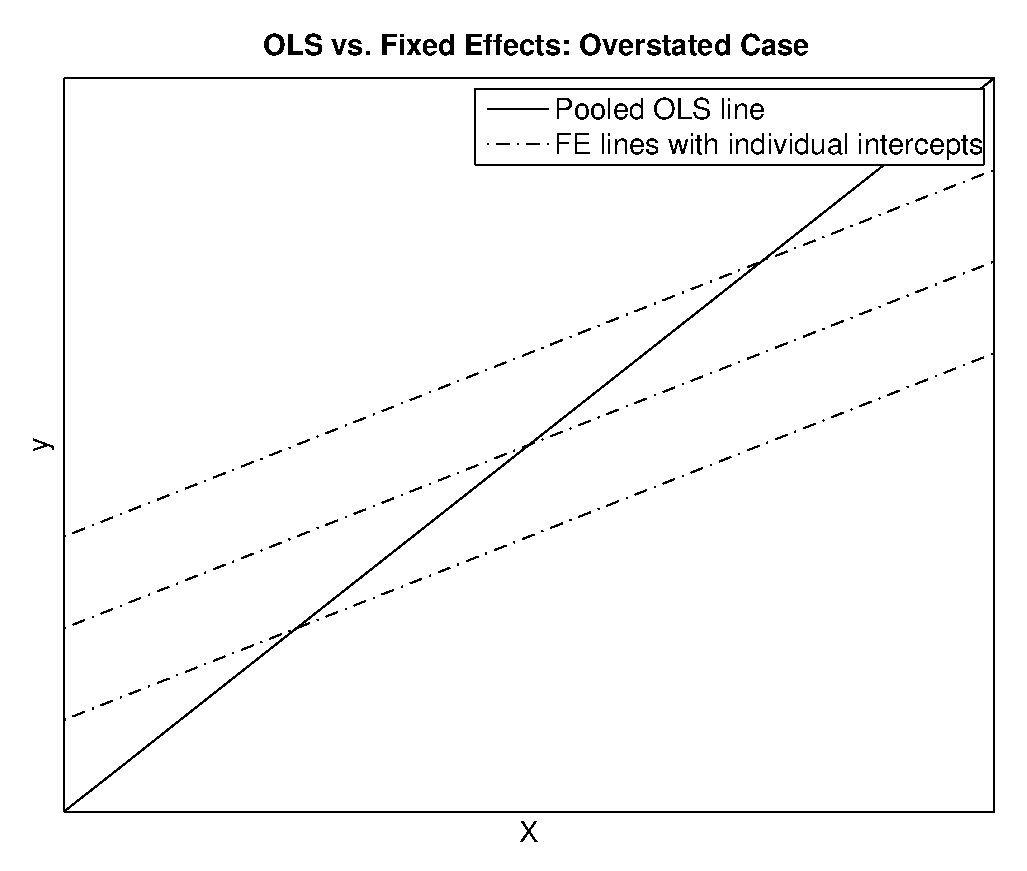
\includegraphics[scale=0.40]{FE_figure1.eps}
\column{3in}
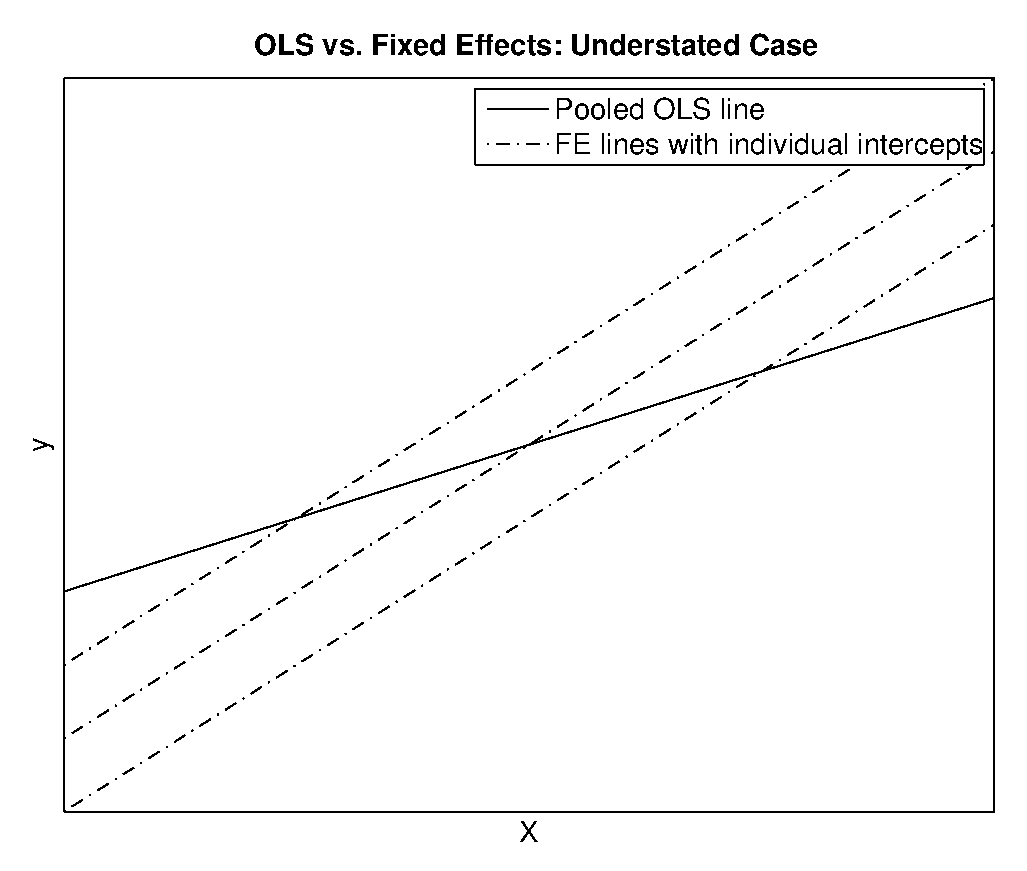
\includegraphics[scale=0.40]{FE_figure2.eps}
\end{columns}
\end{frame}

\begin{frame}
\frametitle{Fixed Effects}
   \bi 
   \item Can also express the fixed effects estimator in a matrix formula: \[
   			 \hat{\beta} = \left(X^{\prime}QX\right)^{-1}X^{\prime} Q y\] where\\ $Q = I_{N}\otimes\left(I_{T}-\frac{1}{T}l_{T}l_{T}^{\prime}\right)$\\ $\otimes$ is the Kronecker Product\\ $l_{T}$ is a $T$-length vector of ones\\ $I_{N}$ is an $N \times N$ identity matrix\\
   \item Notes: This is much more difficult (but not impossible) to implement for panels where $T$ varies across persons (i.e. unbalanced panels). It is also computationally intensive for large $N\ast T$, since $Q$ is a very wide (block diagonal) matrix.
   \ei
\end{frame}

\begin{frame}
\frametitle{Standard Errors of Fixed Effects Estimates}
The variance matrix of $\hat{\beta}$ for fixed effects is 
\[
\hat{\sigma}^{2}_{\varepsilon}\left(\sum_{i=1}^{N}\sum_{t=1}^{T}\ddot{X}_{it}^{\prime}\ddot{X}_{it}\right)^{-1}
\]
where
\[
\hat{\sigma}^{2}_{\varepsilon} = \frac{\textrm{SSR}}{N(T-1)-K}
\]
and where SSR is derived from the sum of the squared residuals from pooled OLS:
\[
\sum_{i}\sum_{t} \left(y_{it}-X_{it}\hat{\beta}_{POLS}\right)^{2}
\]
Note: in matrix form, can estimate \[\textrm{SE}_{\hat{\beta}_{FE}}=\hat{\sigma}^{2}_{\varepsilon}\left(X^{\prime}QX\right)^{-1}\]
\end{frame}

\begin{frame}   
\frametitle{Fixed Effects}
Pros:
      \bi 
      \item Easy to compute
      \item Corrects for permanent unobserved heterogeneity in a straightforward fashion
      \ei
Cons:
      \bi 
      \item Requires panel data
      \item $\beta$ can only be attached to a time-varying $X$ (all time-invariant $X$'s get differenced out)
      \item Specification must be linear
      \item Must assume that heterogeneity is permanent
      \ei
\end{frame}

\begin{frame}
\frametitle{Random Effects}
   \bi 
   \item $y_{it} = X_{it}\beta + \alpha_{i}+ \varepsilon_{it}$
   \item Decompose the error term into a persistent component ($\alpha_{i}$) and a transitory component ($\varepsilon_{it}$) -- both mean-zero
   \item Assume $\varepsilon_{it}$ and $\alpha_{i}$ are each independent of $X_{it}$ and each other for all t
   \item Use variance of $\varepsilon_{it}$ and $\alpha_{i}$ within persons to recover beta:
   \[ \hat{\beta} = \left(\sum_{i=1}^{N} X_{i}^{\prime} \hat{\Omega}^{-1} X_{i}\right)^{-1} \sum_{i=1}^{N}X_{i}^{\prime} \hat{\Omega}^{-1} y_{i}\] where $ \hat{\Omega}^{-1} $ is a matrix of $\hat{\sigma}_{\alpha}^{2}$ and $\hat{\sigma}_{\varepsilon}^{2}$ (variances of the error term components, see Wooldridge p. 259)
   \ei
\end{frame}

\begin{frame}
\frametitle{Random Effects $\hat{\Omega}$ Matrix}
The matrix $\hat{\Omega}$ looks like
\[
\hat{\Omega}_{T \times T}=\left[\begin{array}{cccc}
\hat{\sigma}_{\alpha}^{2}+\hat{\sigma}_{\varepsilon}^{2} & \hat{\sigma}_{\alpha}^{2} & \cdots & \hat{\sigma}_{\alpha}^{2}\\
\hat{\sigma}_{\alpha}^{2} & \hat{\sigma}_{\alpha}^{2}+\hat{\sigma}_{\varepsilon}^{2} &  & \vdots\\
\vdots &  & \ddots & \hat{\sigma}_{\alpha}^{2}\\
\hat{\sigma}_{\alpha}^{2} & \cdots &  & \hat{\sigma}_{\alpha}^{2}+\hat{\sigma}_{\varepsilon}^{2}
\end{array}\right]
\]
where
\[
\hat{\sigma}_{\alpha}^{2}=\frac{1}{NT(T-1)/2-K}\sum_{i=1}^{N}\sum_{t=1}^{T-1}\sum_{s=t+1}^{T}\hat{\hat{u}}_{it}\hat{\hat{u}}_{is}
\]
($\hat{\hat{u}}_{it}$ are pooled OLS residuals), and
\[
\hat{\sigma}_{\varepsilon}^{2}=\left(\frac{1}{NT-K}\sum_{i=1}^{N}\sum_{t=1}^{T}\hat{\hat{u}}_{it}^{2}\right)-\hat{\sigma}_{\alpha}^{2}
\]
\end{frame}

\begin{frame}
\frametitle{Standard Errors of Random Effects Estimates}
The (robust) variance matrix of $\hat{\beta}_{RE}$ (as suggested by Wooldridge (pp. 160, 262) is 
\[
\left(\sum_{i=1}^{N}X_{i}^{\prime}\hat{\Omega}^{-1}X_{i}\right)^{-1}\left(\sum_{i=1}^{N}X_{i}^{\prime}\hat{\Omega}^{-1}\hat{u}_{i}\hat{u}_{i}^{\prime}\hat{\Omega}^{-1}X_{i}\right)\left(\sum_{i=1}^{N}X_{i}^{\prime}\hat{\Omega}^{-1}X_{i}\right)^{-1}
\]
where
where
\[
\hat{u}_{i}=y_{i}-X_{i}\hat{\beta}_{RE}
\]
and where all vectors are of length $T_{i}$ (i.e. number of panels within the individual)
\end{frame}

\begin{frame}{Random Effects}
Pros:
      \bi 
      \item Easy to compute
      \item No differencing, so $\beta$ can be attached to time-invariant $X$'s
      \ei
Cons:
      \bi 
      \item Requires panel data
      \item Requires both error terms to be uncorrelated with $X$ and each other -- strong assumption
      \item Specification must be linear
      \item Must assume that heterogeneity is permanent
      \ei
\end{frame}

\begin{frame}
\frametitle{Fixed Effects vs. Random Effects}
   \bi 
   \item Random effects is more efficient, but fixed effects is more robust
   \item i.e. if $\alpha_{i}$ and $\varepsilon_{it}$ are actually independent, RE will give smaller standard errors
   \item However, if this is not true, RE is inconsistent so FE should be used
   \item Researcher can use a Hausman test to see if RE should be used
   \item In practice, most papers use FE because it's easier to understand, requires fewer assumptions, and is more robust to misspecification
   \ei
\end{frame}

\begin{frame}
\frametitle{Unobserved Heterogeneity in Nonlinear Models}
   \bi 
   \item So far, we've only looked at unobserved heterogeneity in linear models
   \item Once the model becomes nonlinear (e.g. simple probit), it becomes increasingly difficult to correct for unobserved heterogeneity because differencing won't work
   \item Can't easily do fixed effects in nonlinear models (no differencing, and dummy for each person $\Rightarrow$ incidental parameters problem)
   \item Random effects is easier to compute, but requires additional assumptions and is inconsistent if the effect is actually correlated with $X$
   \ei
\end{frame}

\begin{frame}
\frametitle{Unobserved Heterogeneity in MLE Models}
   \bi 
   \item Most MLE models assume a random effects specification for the unobserved heterogeneity
   \item Assume a distribution of the RE (e.g. normal, discrete-non-parametric) 
   \item Integrate out the unobserved effect from the likelihood while recovering parameters that characterize the assumed distribution
   \item Some fancier models can estimate heterogeneity that is both permanent and transitory (something FE/RE can't do)
      \bi 
      \item This requires more elaborate assumptions
      \ei
   \item You'll learn more about the finer points of this in your 2nd year modules
   \ei
\end{frame}

\begin{frame}
\frametitle{Unobserved Heterogeneity in Perspective}
   \bi 
   \item Estimation results that have corrected for unobserved heterogeneity are more important than any other estimation results
   \item You will not be able to publish anything without saying  \emph{something} about unobserved heterogeneity
   \item At the end of the day, it doesn't matter too much  \emph{how} you make the correction, just  \emph{that} you make the correction
   \ei
\end{frame}
\end{document}
